\setAuthor{Mihkel Kree}
\setRound{lõppvoor}
\setYear{2007}
\setNumber{G 9}
\setDifficulty{9}
\setTopic{Geomeetriline optika}

\prob{Nõguspeegel}
Optiline süsteem koosneb kumerläätsest ja nõguspeeglist, mille optilised peateljed ühtivad. Kumerpeegli asukohta pole joonisel märgitud. On teada, et objektist $A$ tekib teisele poole läätse kaks kujutist $K_1$ ja $K_2$. Konstrueerige kumerpeegli kõveruskeskpunkt $O$ ja kumerpeeglis objektist $A$ tekkinud näiv kujutis $A'$. Eeldada, et optilises süsteemis on nurgad piisavalt väiksed, et sfäärilisi aberratsioone ei teki.

\begin{center}
	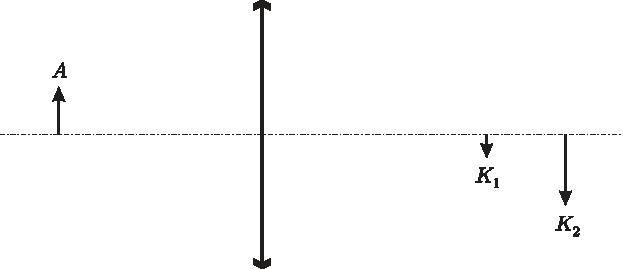
\includegraphics[width=\linewidth]{2007-v3g-09-yl}
\end{center}

\hint
Kahe kujutamise tekkeks peab kumerpeegel asuma objektist $A$ vasakul. $A'$ leidmiseks peab määrama läätse fookuse, aga selleks peab silmas pidama asjaolu, et pole teada, kumb kujutistest $K_1$ ja $K_2$ kuulub objektile $A$.

\solu
Paneme tähele, et kõverustsenter $O$, objekt $A$ ning kujutis $A'$ kumerpeeglis asuvad samal sirgel. Seega, kui meil õnnestub leida sirge $AA'$, siis selle lõikepunkt optilise teljega annaks punkti $O$. Teisest küljest, kiir, mis läbib punkti $A$ kujutist läätses, $K_2$, ja punkti $A'$ kujutist, $K_1$, jätkub peale murdumist läätses sirgena $s'$ ja läbib nii punkti $A$ kui $A'$. Tänu sellele leiamegi sirge $AA'$ ja punkti $O$.

Punkti $A'$ leidmiseks konstrueerime esmalt fokaaltasandi $F$. Selleks leiame fokaaltasandis lebava punkti --- sirge $s$ lõikepunkti sirgega $t$, mis on paralleelne sirgega $s'$ ja läbib läätse keskpunkti. Kujutisi $K_1$ ja $K_2$ ühendav sirge murdub nii, et selle pikenduse lõikepunkt optilise peateljega ongi otsitav kõverustsenter. Punkti $A'$ leiame kui sirge $s'$ lõikepunkti sirgega $q'$, mis peale murdumist läbib fookuse ja punkti $K_1$ (sest $K_1$ on $A'$ kujutiseks).


\begin{center}
	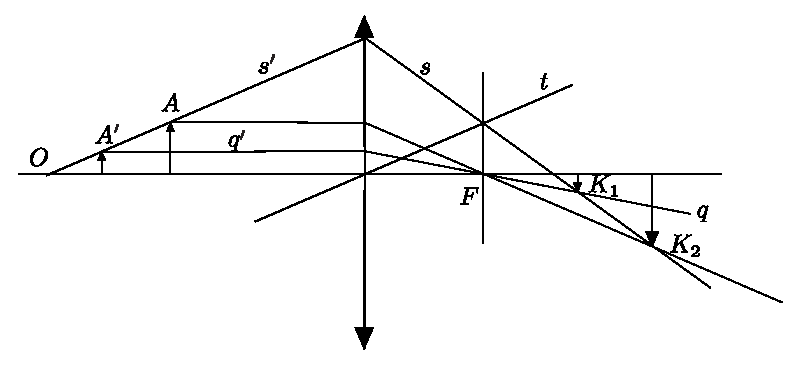
\includegraphics[width=\linewidth]{2007-v3g-09-lah}
\end{center}
\probend